This assignment asks to get the equations of motion using the Hamilton Principle:
\begin{equation}
    \begin{split}
        \int_{t_1}^{t_2}\delta(T-V+W)dt = 0
    \end{split}
\end{equation}

Using the theory discussed in the lecture we can split the term into different contributions::

% \begin{equation}
%     \begin{split}
%         \int_{t_1}^{t_2}\int_0^L \left[
%             \underbrace{\frac{\partial L}{\partial q} \delta q}_{A} + 
%             \underbrace{\frac{\partial L}{\partial q'}\delta q'}_{B} + 
%             \underbrace{\frac{\partial L}{\partial q''}\delta q''}_{C} + 
%             \underbrace{\frac{\partial L}{\partial \dot q} \delta \dot q}_{D} + 
%             \underbrace{\frac{\partial L}{\partial \dot q'} \delta \dot q'}_{E}+ 
%             \delta \text{W}\right]dxdt 
%     \end{split}
% \end{equation}
% \begin{equation}
%     \begin{split}
%         &\frac{\partial L}{\partial w} - \frac{\partial}{\partial x}\left(\frac
%         {\partial L}{w'}\right) + \frac{\partial ^2}{\partial x^2}\left(\frac
%         {\partial L}{\partial w''}\right) - \frac{\partial}{\partial t}\left(\frac{\partial L}{\partial \dot w}\right) + \frac{\partial }{\partial x}\left(\frac{\partial}{\partial t}\left(\frac{\partial L}{\partial \dot w'}\right)\right) + p(x,t) = 0\\
%         &x \in [0;L]
%     \end{split}
% \end{equation}

Remembering the result of the Hamilton principle from the lecture:

\begin{figure}[ht]
    \centering
    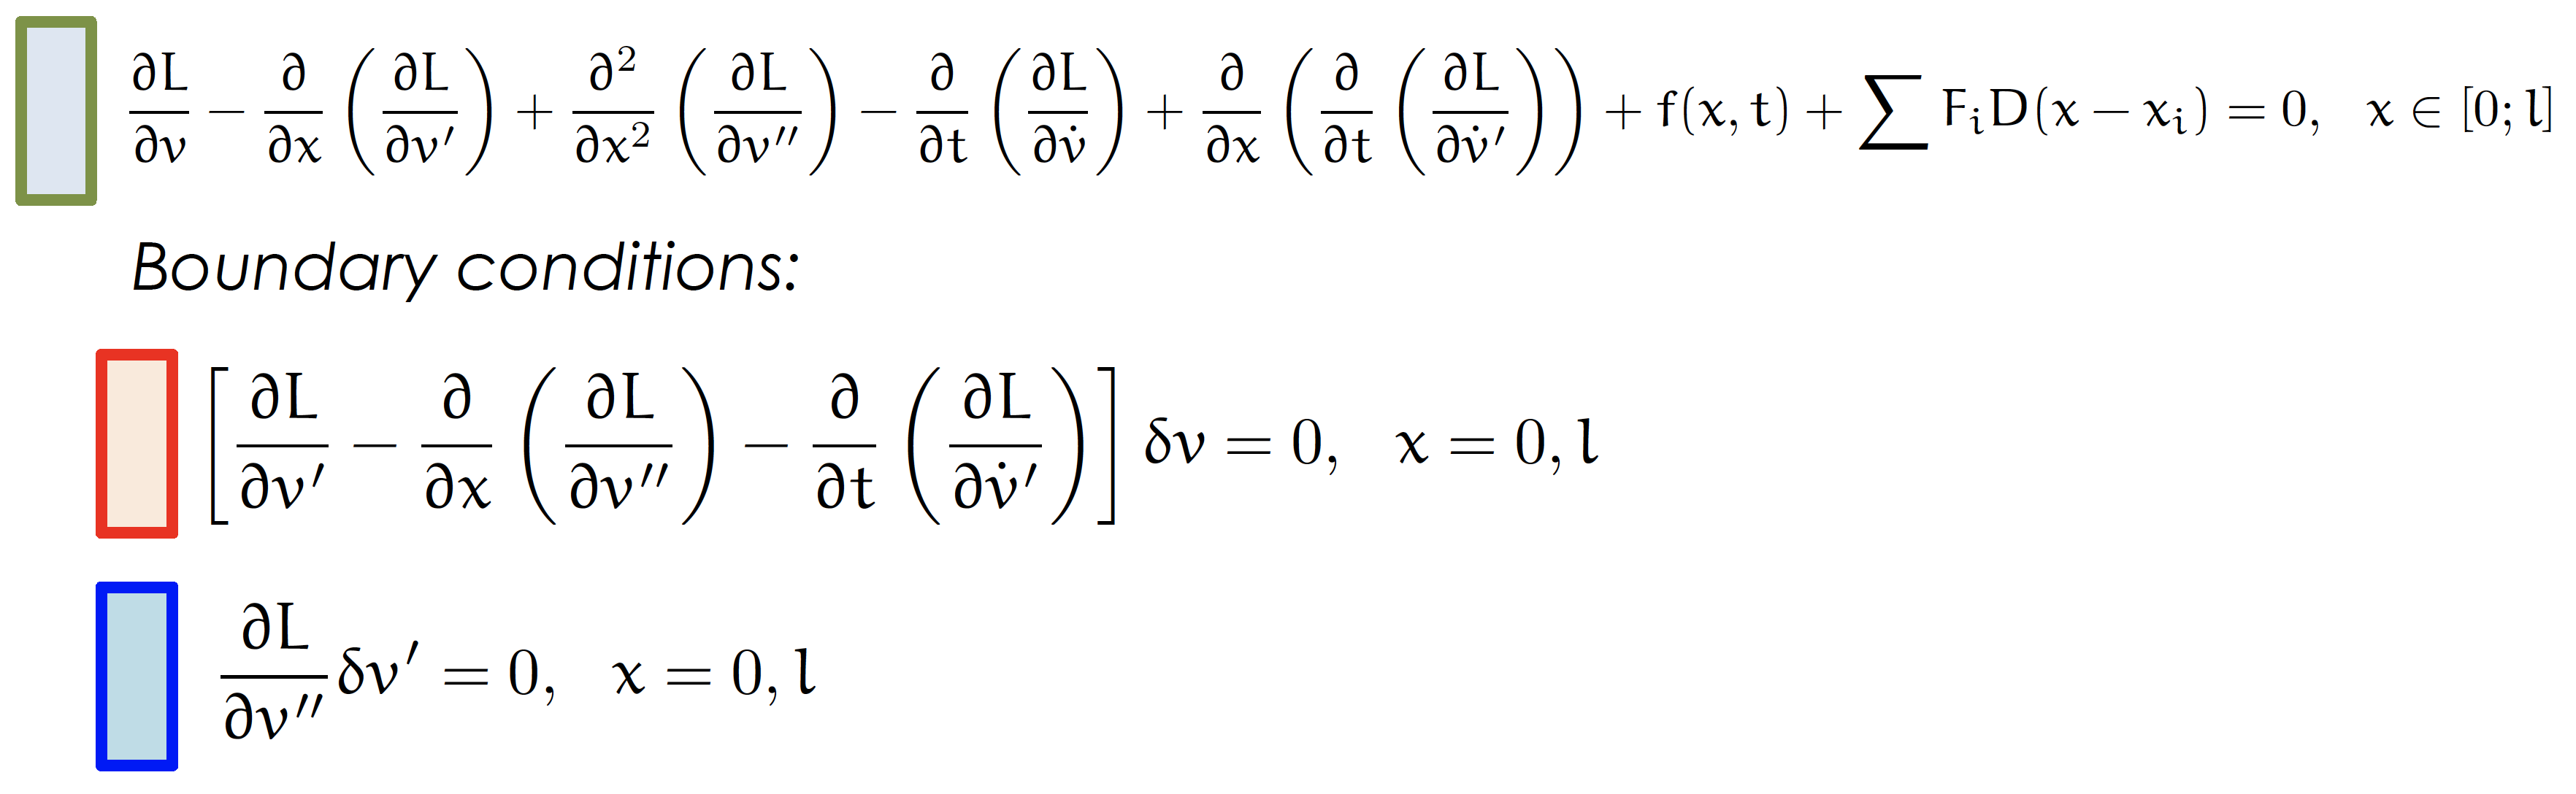
\includegraphics[scale=0.2]{images/Hamilton.png}
    \caption{Hamilton Formulas for a continuous system}
    %label always in the end
    \label{fig:hamilton}
\end{figure}

We consider w our variable instead of v.

\begin{equation}
    \begin{split}
        &\frac{\partial L}{\partial w} = 0, \quad \frac{\partial}{\partial x}\frac{\partial L}{\partial w'} = 0, \quad    
    \end{split}
\end{equation}

\begin{equation}
    \begin{split}
        &\frac{\partial^2}{\partial x^2}\frac{\partial L}{\partial w''} = -E\frac{\partial^2}{\partial x^2}I(x), \hspace{0.5cm} \frac{\partial}{\partial t}\frac{\partial L}{\partial \dot w} = 2\delta A(x)\ddot w, \hspace{0.5cm}
    \end{split}
\end{equation}

\begin{equation}
    \begin{split}
        &\frac{\partial}{\partial x}\left(\frac{\partial}{\partial t}\left(\frac{\partial L}{\partial \dot w'}\right)\right) = 2\rho I(x) \ddot w'' + 2\rho I(x)' \ddot w'
    \end{split}
\end{equation}

\begin{equation}
    \begin{split}
        f(x,t) = p(x,t)
    \end{split}
\end{equation}

Therefore the green part comes to:

While for the red we get:

And for lastly for the blue:


